\documentclass[conference]{IEEEtran}
\IEEEoverridecommandlockouts
\usepackage{}
\usepackage{cite}
\usepackage{amsmath,amssymb,amsfonts}
\usepackage{algorithm}
\usepackage{algorithmic}
\usepackage{float}
\usepackage{graphicx}
\usepackage{textcomp}
\usepackage{xcolor}
\def\BibTeX{{\rm B\kern-.05em{\sc i\kern-.025em b}\kern-.08em
    T\kern-.1667em\lower.7ex\hbox{E}\kern-.125emX}}
\begin{document}

\title{Autonomous UAV Localization via Aerial-to-Satellite Image Registration: Interim Report\\
}

\author{
\IEEEauthorblockN{Solomiia Gadiichuk}
\IEEEauthorblockA{\textit{Faculty of Applied Sciences} \\
Ukrainian Catholic University\\
Lviv, Ukraine \\
hadiichuk.pn@ucu.edu.ua}
\and
\IEEEauthorblockN{Bohdan Zasymovych}
\IEEEauthorblockA{\textit{Faculty of Applied Sciences} \\
Ukrainian Catholic University\\
Lviv, Ukraine\\
zasymovych.pn@ucu.edu.ua}
\and
\IEEEauthorblockN{Marta Kosiv}
\IEEEauthorblockA{\textit{Faculty of Applied Sciences} \\
Ukrainian Catholic University\\
Lviv, Ukraine\\
kosiv.pn@ucu.edu.ua}
}

\maketitle

\begin{abstract}
Navigating Unmanned Aerial Vehicles (UAVs) in GNSS-denied environments is a critical challenge due to the massive deployment of Electronic Warfare systems. When satellite navigation fails, autonomous systems need reliable alternatives for absolute positioning. This project develops a vision-based localization engine that calculates a UAV's geographic coordinates by matching its real-time camera feed against preloaded satellite maps. The pipeline uses SIFT for feature extraction and RANSAC for geometric outlier rejection to estimate an Affine transformation between images. The estimated model then projects the drone's optical center onto the global coordinate plane.
\end{abstract}

\begin{IEEEkeywords}
UAV Localization, GNSS-denied Navigation, Image Registration, Feature Matching, Affine Transformation, RANSAC, SIFT
\end{IEEEkeywords}

\section{Introduction}
Visual Unmanned Aerial Vehicle (UAV) localization enables autonomous flight by calculating absolute geographic coordinates solely from optical sensors. This involves matching the UAV's real-time images against georeferenced satellite maps.

\begin{figure}[htbp]
    \centering
    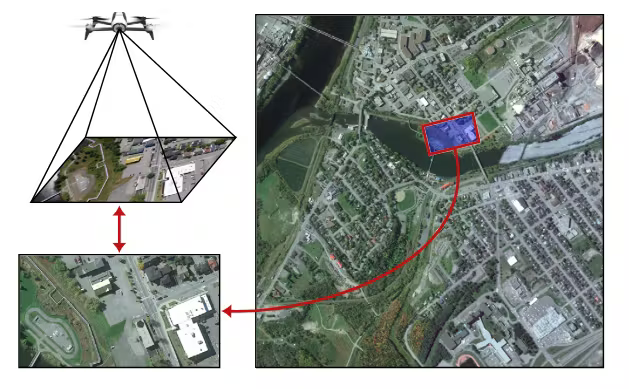
\includegraphics[width=1\columnwidth]{figs/image_to_map_localization.png}
    \caption{Matching the UAV camera feed to a reference satellite map \cite{b1}.}
    \label{fig:image_to_map}
\end{figure}

These systems are critical in modern warfare, where Electronic Warfare (EW) makes Global Navigation Satellite Systems (GNSS) highly vulnerable. Vision-based localization offers a passive, unjammable alternative, allowing UAVs to compute coordinates from onboard visual data and navigate GNSS-denied environments.

This project develops an automated vision-based positioning system for UAVs. To achieve this goal, the software pipeline is broken down into the following objectives:
\begin{itemize}
    \item \textbf{Feature Extraction:} Detect and describe geometric keypoints in both images using the OpenCV SIFT algorithm.
    \item \textbf{Feature Matching:} Match descriptors using nearest-neighbor search filtered by Lowe's ratio test.
    \item \textbf{Outlier Rejection:} Use RANSAC to filter false matches and identify a geometrically consistent consensus set.
    \item \textbf{Transformation Estimation:} Compute an optimal 6-degree-of-freedom Affine transformation using least-squares to map the images.
    \item \textbf{Coordinate Projection:} Apply the Affine transformation to the UAV image center to calculate the drone's absolute position.
\end{itemize}

\section{Related Work}

\subsection{Absolute Visual Localization Approaches}
As outlined in \cite{b1}, vision-based localization includes map-independent methods (estimating relative motion with drift) and map-based methods (providing drift-free absolute coordinates). For map-based UAV-to-satellite registration, there are three primary paradigms:

\begin{itemize}
    \item \textbf{Direct Template Matching:} Slides the real-time image across the reference map to find the highest raw pixel correlation.
    \item \textbf{Feature-Point Matching:} Extracts distinct geometric interest points and matches their mathematical descriptors.
    \item \textbf{Deep Learning-Based Matching:} Uses neural networks to extract high-level semantic context.
\end{itemize}

Template matching compares raw pixels, making it fast but sensitive to scale and rotation. Feature matching extracts geometric keypoints, ensuring robustness against tilt and altitude changes. Deep learning evaluates semantic context, handling extreme variations at high computational costs.

\subsection{Keypoint Detection and Description}
Feature detection computes abstractions of image information. Based on \cite{b2}, the primary traditional algorithms are:

\begin{itemize}
    \item \textbf{SIFT:} Uses Difference of Gaussian for scale-space extrema estimation and descriptor generation. While computationally complex, it is highly robust against rotation and affine transformations.
    \item \textbf{SURF:} Approximates the Difference of Gaussian with box filters. It performs faster than SIFT while maintaining detection quality.
    \item \textbf{ORB:} A fusion of FAST and BRIEF. It is the fastest algorithm but more sensitive to certain transformations than SIFT.
\end{itemize}

While ORB is faster, SIFT achieves higher matching rates across most transformations, including intensity, rotation, shearing, and fisheye distortion \cite{b2}. SIFT is selected for this project due to this robustness.

\subsection{Geometric Transformations}
Geometric transformations define the mathematical mapping between UAV imagery and the reference map. We consider three linear models:

\begin{itemize}
    \item \textbf{Similarity Transformation:} A 4-degree-of-freedom model accounting for translation, rotation, and uniform scaling.
    \item \textbf{Affine Transformation:} A 6-degree-of-freedom model extending similarity by adding shear and non-uniform scaling.
    \item \textbf{Projective:} An 8-degree-of-freedom model representing the true 3D to 2D projection.
\end{itemize}

The Similarity model requires perfectly level flight and uniform zooming, failing with axial stretching or tilt. The Affine model approximates slight perspective shifts via shear, but only the Projective model handles significant pitch and roll by modeling converging parallel lines. 

We chose the Affine model because it flexibly handles non-ideal conditions (slight tilt or shearing) while remaining mathematically simpler and more stable than the Projective model.


\section{Proposed Methodology and Implementation}

\subsection{Mathematical Formulation}
The mapping between the UAV image coordinates $(x, y)$ and the map coordinates $(X, Y)$ is modeled by an Affine transformation. This is represented by a $3 \times 3$ matrix where the third row is fixed to $(0, 0, 1)$ to preserve affine properties:
\begin{equation}
\begin{bmatrix} X \\ Y \\ 1 \end{bmatrix} = \begin{bmatrix} a_1 & a_2 & t_x \\ a_3 & a_4 & t_y \\ 0 & 0 & 1 \end{bmatrix} \begin{bmatrix} x \\ y \\ 1 \end{bmatrix}
\end{equation}

To estimate these parameters, we utilize the RANSAC algorithm. In each iteration, RANSAC generates a transformation hypothesis from a minimal sample and calculates the number of inliers based on an error $d$:
\begin{equation}
d = \sqrt{(X_i - \hat{X}_i)^2 + (Y_i - \hat{Y}_i)^2} < \epsilon
\end{equation}
The algorithm selects the matrix that yields the greatest number of inliers. All remaining points classified as outliers for this specific matrix are discarded.

Once the optimal consensus set of $n$ inliers is identified, we define an overdetermined system $A\mathbf{v} = \mathbf{b}$ where $\mathbf{v} = [a_1, a_2, t_x, a_3, a_4, t_y]^T$:
\begin{equation}
\begin{bmatrix} 
x_1 & y_1 & 1 & 0 & 0 & 0 \\ 
0 & 0 & 0 & x_1 & y_1 & 1 \\ 
\vdots & \vdots & \vdots & \vdots & \vdots & \vdots \\ 
x_n & y_n & 1 & 0 & 0 & 0 \\ 
0 & 0 & 0 & x_n & y_n & 1 
\end{bmatrix} 
\begin{bmatrix} a_1 \\ a_2 \\ t_x \\ a_3 \\ a_4 \\ t_y \end{bmatrix} = 
\begin{bmatrix} X_1 \\ Y_1 \\ \vdots \\ X_n \\ Y_n \end{bmatrix}
\end{equation}

The optimal solution $\mathbf{v}_{final}$ is the one that minimizes the sum of squared residuals, defined by the cost function $J(\mathbf{v})$:
\begin{equation}
J(\mathbf{v}) = \|A\mathbf{v} - \mathbf{b}\|^2 = (A\mathbf{v} - \mathbf{b})^T(A\mathbf{v} - \mathbf{b})
\end{equation}

Expanding the terms, we obtain:
\begin{equation}
J(\mathbf{v}) = \mathbf{v}^T A^T A \mathbf{v} - 2\mathbf{b}^T A \mathbf{v} + \mathbf{b}^T \mathbf{b}
\end{equation}

To find the minimum, we compute the derivative with respect to $\mathbf{v}$ and set it to zero:
\begin{equation}
\frac{\partial J(\mathbf{v})}{\partial \mathbf{v}} = 2A^T A \mathbf{v} - 2A^T \mathbf{b} = 0
\end{equation}

Solving this linear equation yields the final parameter vector:
\begin{equation}
A^T A \mathbf{v} = A^T \mathbf{b} \implies \mathbf{v}_{final} = (A^T A)^{-1} A^T \mathbf{b}
\end{equation}

\subsection{Algorithmic Pipeline}

\begin{algorithm}[H]
\caption{UAV Localization Pipeline}
\begin{algorithmic}[1]
\REQUIRE UAV Image $I_{uav}$, Reference Map $I_{map}$
\ENSURE Global Coordinates $(X_{map}, Y_{map})$
\STATE Convert $I_{uav}$ and $I_{map}$ to the grayscale.
\STATE Extract SIFT features and match using Lowe's ratio test.
\STATE \textbf{while} $i < max\_iterations$ \textbf{do}
\STATE \quad Sample 3 random pairs and compute $M_{temp}$.
\STATE \quad Count inliers satisfying $d < \epsilon$.
\STATE \quad If current consensus is the largest, store $M_{temp}$ and inliers.
\STATE \textbf{end while}
\STATE Solve the overdetermined system using all stored inliers.
\STATE Project UAV center $(x_c, y_c, 1)$ to get $(X_{map}, Y_{map})$.
\RETURN $(X_{map}, Y_{map})$
\end{algorithmic}
\end{algorithm}

\section{Evaluation Strategy}
To validate the system, we will test it on a synthetic dataset derived from high-resolution satellite imagery. UAV camera feeds will be artificially generated by applying geometric deformations (scaling, rotation, shearing), noise, and color distortion to simulate real conditions.

The primary metric for accuracy will be the Root Mean Square Error (RMSE), which measures the Euclidean distance between the estimated coordinates $(\hat{X}, \hat{Y})$ and the known ground-truth coordinates $(X, Y)$ across $N$ test frames:
\begin{equation}
RMSE = \sqrt{\frac{1}{N} \sum_{i=1}^{N} \left( (X_{i} - \hat{X}_{i})^2 + (Y_{i} - \hat{Y}_{i})^2 \right)}
\end{equation}
Additionally, we will evaluate total and average execution times to estimate whether our pipeline is suitable for real-time UAV localization.

\section{Project Roadmap and Risk Analysis}
Remaining work to complete the prototype is divided into three phases over six weeks:

\subsection{Timeline}

\begin{itemize}
    \item \textbf{Week 1-3 (Implementation):} Implement the full algorithm pipeline: image loading, preprocessing, SIFT, RANSAC, and final coordinate estimation.
    \item \textbf{Week 4-5 (Testing \& Evaluation):} Find suitable satellite images, generate synthetic UAV datasets, and run tests to compute RMSE and execution times.
    \item \textbf{Week 6 (Improvements):} If time permits, we plan to test a Projective transformation to account for non-parallel camera angles. We will also seek real-world datasets to evaluate the model on actual flight data.
\end{itemize}

\subsection{Risk Analysis}
A primary risk is poor model performance during evaluation. While theoretically sound, the implementation may lack robustness for real-world conditions, causing high errors. If the algorithm underperforms, we will reconsider our methodology and explore alternatives, like different feature extraction methods or upgrading to a Projective transformation model.

\begin{thebibliography}{00}
\bibitem{b1} Encord, ``Vision-Based Localization: A Guide to VBL Technique.'' [Online]. Available: https://encord.com/blog/vision-based-localization-a-guide-to-vbl-technique/
\bibitem{b2} E. Karami, S. Prasad, and M. Shehata, ``Image Matching Using SIFT, SURF, BRIEF and ORB: Performance Comparison for Distorted Images,'' arXiv preprint arXiv:1710.02726, 2017. [Online]. Available: https://arxiv.org/abs/1710.02726
\end{thebibliography}

\end{document}
